
\section*{Simulado 1}

\num{1} O número de ouro é um número misterioso e enigmático presente em uma
infinidade de elementos da natureza na forma de uma razão que é
considerada por muitos como a divina proporção ou razão divina.

Seu valor é:

(\frac{1 + \ \sqrt{5}}{2}) = 1,6180339887...

Como podemos definir esse número?
\item Irracional
\item Racional
\item Inteiro
\item Natural

% SAEB: Identificar números racionais ou irracionais. BNCC: F09MA02 --
% Reconhecer um número irracional como um número real cuja representação
% decimal é infinita e não periódica, e estimar a localização de alguns
% deles na reta numérica.

% A: Correta, pois se trata de um número irracional.

% B: Incorreta, pois não se trata de um número racional.

% C: Incorreta, pois não se trata de um número inteiro.

% D: Incorreta, pois não se trata de um número natural.

\num{2} Durante seus estudos, um físico descobriu que a massa de um elétron
pesa aproximadamente 0,000000000000000000000000000911 g. Outra forma
válida de representarmos esse número é
\item (9,11 \cdot 10^{-29})
\item (9,11 \cdot 10^{-28})
\item ( 9,11 \cdot 10^{-27})
\item (9,11 \cdot 10^{-26})

% SAEB: Resolver problemas de adição, subtração, multiplicação, divisão,
% potenciação ou radiciação envolvendo número reais, inclusive notação
% científica.

% BNCC: EF08MA01 -- Efetuar cálculos com potências de expoentes inteiros e
% aplicar esse conhecimento na representação de números em notação
% científica.

% A: Incorreta, pois, ao contar um ``zero'' a mais, o aluno chegaria a
% esse resultado.

% B: Correta, pois, utilizando a notação científica, temos que:

% 0,000000000000000000000000000911,

% 30 casas após a vírgula; logo, é necessário o deslocamento do primeiro
% número após o 0:

% (0,000000000000000000000000000911 = 9,11 \cdot 10^{-28})

% C: Incorreta, pois, ao contar um ``zero'' a menos, o aluno chegaria a
% esse resultado.

% D: Incorreta, pois, ao contar dois ``zeros'' a menos, o aluno chegaria a
% esse resultado.

\num{3} Em um festival de música, a capacidade total de público era de 50.000
pessoas. Sabendo que (\frac{99}{100}) do público total compareceu,
qual foi a capacidade atingida nesse festival?
\item 49.999
\item 49.500
\item 49.001
\item 4.950

% SAEB: Representar frações menores ou maiores que a unidade por meio de
% representações pictóricas ou associar frações a representações
% pictóricas.

% A: Incorreta, pois o aluno pode chegar à conclusão de que 100 - 99 = 1.

% B: Correta, pois, realizando o Cálculo, temos que
% ( \frac{50.000} {100} = 500)

% 500 \cdot 99 = 49.500.

% C: Incorreta, pois o aluno pode considerar retirar 99 do valor de 50.000
% e chegar ao resultado da alternativa descrita.

% D: Incorreta, pois o aluno pode chegar a esse resultado realizando a
% multiplicação por 0,099.

\num{4} João paga R\$\,4,25 por uma passagem de ônibus. Ele ficou sabendo que
esse preço terá um aumento de 12\%. Quanto João passará a pagar pela
passagem?
\item 0,51
\item 3,74
\item 4,37
\item 4,76

% SAEB: Resolver problemas que envolvam porcentagens, incluindo os que
% lidam com acréscimos e decréscimos simples, aplicação de percentuais
% sucessivos e determinação de taxas percentuais.

% BNCC: EF08MA04 -- Resolver e elaborar problemas, envolvendo cálculo de
% porcentagens, incluindo o uso de tecnologias digitais.

% A: Incorreta, pois esse seria o acréscimo do valor da passagem, e não o
% valor final.

% B: Incorreta, pois esse seria o valor da passagem caso ocorresse 12\% de
% desconto.

% C:Incorreta, pois o aluno pchegaria a esse valor caso somasse os dois
% números.

% D: Correta, pois

% (\frac{4,25}{x} \cdot \frac{100}{112})

% 4,25 \cdot 112 = x \cdot 100

% 476= 100x

% X = 4,76

\num{5} Maria tem em seu carro R$\,15,60 em moedas de R$ 0,10 e de R\$\,0,25.
Tento em vista que o número de moedas de 25 centavos é o dobro do número
de moedas de 10 centavos, o total de moedas é?
\item 52
\item 26
\item 1 352
\item 78

% SAEB: Resolver problemas que possam ser representados por sistema de
% equações de 1º grau com duas incógnitas.

% A: Incorreta, pois o aluno pode considerar o valor parcial como o valor
% final do número de moedas.

% B: pois o aluno pode considerar o valor parcial como o valor final do
% número de moedas.

% C: Incorreta, pois o aluno pode realizar a multipicação ao invés da
% soma.

% D: Correta, pois, lendo o enunciado, obtemos o seguinte sistema de
% equações:

% 0,25x + 10y = 15,60

% X = 2y

% Logo, já conseguimos substituir a 2ª. equação na primeira

% 0,25 \cdot 2y + 0,10y = 15,60

% 0,50y + 0,10y = 15,60

% 0,60y = 15,60

% Y = 26

% Como x é o dobro de y, temos: x = 2y = 2 \cdot 26 = 52

\num{6} Arlindo resolveu presentear sua filha com 2 caixas de tamanhos
diferentes. Arlindo pretende enchê-las com joias. Qual é a equação que
representa o volume máximo de joias que a filha de Arlindo vai receber
somando o volume das duas caixas? EF08MA10 - Resolver problemas que
envolvam cálculo do valor numérico de expressões algébricas.

\begin{figure}[H]
\centering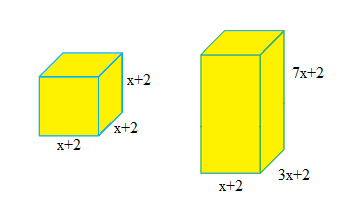
\includegraphics[width=2.63333in,height=1.56545in]{./imgSAEB_8_MAT/media/image55.png}
\end{figure}
\item X^3 + 6x^2 + 12x + 8
\item 21x^3 + 62x^2 + 44x + 8
\item 22x^3 + 68x^2+ 56x
\item 22x^3 + 68x^2 + 56x + 16

% SAEB: Resolver problemas que envolvam volume de prismas retos ou
% cilindros retos.

% BNCC: EF08MA21 -- Resolver e elaborar problemas que envolvam o cálculo
% do volume de recipiente cujo formato é o de um bloco retangular.

% A: incorreta o aluno poderia chegar a essa conclusão chegando apenas ao
% valor do volume apenas da primeira caixa.

% B: incorreta o aluno poderia chegar a essa conclusão chegando apenas ao
% valor do volume apenas da segunda caixa.

% C: o aluno chegaria a esse valor calculando incorretamente o ultimo
% termo da equação esquecendo de realizar a última parte valor numérico

% D: Correta, pois, considerando a fórmula do cálculo do volume, temos
% que:

% 1ª. caixa

% (x+2) \cdot (x+2) \cdot (x+2) =

% (X^2 + 2x + 2x + 4) \cdot (x + 2) =

% (x^2 + 4x + 4) \cdot (x + 2) =

% X^3 + 2x^2 + 4x^2 + 8x + 4x + 8 =

% X^3 + 6x^2 + 12x + 8

% 2ª. caixa

% (x + 2) \cdot (3x + 2) \cdot (7x + 2)=

% (3x^2 +2x + 6x + 4) \cdot (7x + 2)=

% (3x^2 + 8x + 4 ) \cdot (7x + 2)=

% 21x^3 + 6x^2 + 56x^2 + 16x + 28x + 8=

% 21x^3 + 62x^2 + 44x + 8

% Somando o valor das 2 caixas, temos que

% X^3 + 6x^2 + 12x +8 + 21x^3 + 62x^2 + 44x + 8 =

% 22x^3 + 68x^2 + 56x + 16

\num{7} Josué é estudante de cálculo em uma faculdade de sua cidade. Certo
dia, ele resolveu calcular quantos segundos demora caminhando de um lado
para o outro em sua casa, e chegou à conclusão de que o tempo em
segundos é determinado pela formula t^2 - 36 = 0. Sendo assim, quanto
tempo Josué demora para atravessar de um lado para o outro na casa?
\item 36
\item 6
\item 37
\item 2

% SAEB: Resolver problemas que possam ser representados por equações
% polinomiais de 2º grau.

% BNCC: EF08MA09 -- Resolver e elaborar, com e sem uso de tecnologias,
% problemas que possam ser representados por equações polinomiais de 2º
% grau do tipo ax2 = b.

% a: Incorreta, pois esse valor representa apenas um dos termos da
% equação.

% b: Correta, pois, realizando a operação, obtemos:

% t^2 - 36 = 0

% t^2 = (\sqrt{36})

% t = ± 6

% C: Incorreta, pois o aluno pode chegar a esse valor somando todos os
% termos da equação.

% D: Incorreta, pois o aluno pode apenas retirar o termo quadrático e
% cogitar que essa possa ser a alternativa correta.

\num{8} Helena resolveu visitar seus pais que moram a 455 km de distância de
sua cidade. Helena chegou 7 horas após sair de sua casa. Qual foi a
velocidade média que Helena obteve nesse percurso?
\item 65 km/h
\item 7,56 km/h
\item 1,08 km/h
\item 18,05 km/h

% SAEB: Resolver problemas que envolvam variação de proporcionalidade
% direta ou inversa entre duas ou mais grandezas, inclusive escalas,
% divisões proporcionais e taxa de variação.

% BNCC: EF08MA12 -- Identificar a natureza da variação de duas grandezas,
% diretamente, inversamente proporcionais ou não proporcionais,
% expressando a relação existente por meio de sentença algébrica e
% representá-la no plano cartesiano.

% A: Correta, pois, utilizando a razão (\frac{distância}{\text{tempo}}),
% temos que (\frac{455}{7}) = 65km/h

% A velocidade média desse carro foi de 65 km/h.

% B: Incorreta, pois o aluno pode chegar a essa conclusão caso divida a
% distância pelo valor de 60 minutos ao invés de 7 horas.

% C: Incorreta, pois o aluno chegará a essa conclusão confundindo km/h por
% km/m.

% D: Incorreta, pois o aluno chegará a essa conclusão confundindo km/h por
% m/s.

\num{9} Considerando a figura abaixo, em que ABC é a representação de um
triângulo equilátero, calcule a medida do ângulo x.
\begin{figure}[H]
\centering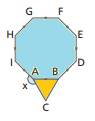
\includegraphics[width=0.98958in,height=1.26042in]{./imgSAEB_8_MAT/media/image56.png}
\end{figure}
\item 135°
\item 165°
\item 60°
\item 300°

% SAEB: Relacionar o número de vértices, faces ou arestas de prismas ou
% pirâmides, em função do seu polígono da base.

% BNCC: EF08MA18 -- Reconhecer e construir figuras obtidas por composições
% de transformações geométricas (translação, reflexão e rotação), com o
% uso de instrumentos de desenho ou de softwares de geometria dinâmica.

% A: Incorreta, pois o aluno chegaria a essa conclusão realizando apenas a
% primeira parte do cálculo.

% B: Correta, pois, utilizando a fórmula para obter o valor da figura,
% temos que:

% (\frac{Ai = \left( 8 - 2 \right)\ \ .\ \ 180}{8}) =

% (\frac{Ai = \ 6\ \ .\ \ 180}{8\ }) =

% (\frac{Ai = 1080}{8}) = 135°

% Calculando os ângulos do triângulo:

% (\frac{Ai = \left( 3 - 2 \right)\ \ .\ \ 180}{3}) =

% (\frac{Ai = \ \ \ 180}{3}) = 60°

% C: Incorreta, pois o aluno pode considerar o valor do ângulo interno do
% triângulo como resposta, o que é incorreto.

% D: Incorreta, pois o aluno chegaria a esse valor caso não subtraísse
% também o valor do ângulo do triângulo.

\num{10} As medidas dos ângulos de um triângulo são expressas, em graus, por:
3x, 4x + 15° e 6x - 30°. Qual é a medida do ângulo maior?
\item 45°
\item 60°
\item 75°
\item 180°

% SAEB: Resolver problemas que envolvam relações entre ângulos formados
% por retas paralelas cortadas por uma transversal, ângulos internos ou
% externos de polígonos ou cevianas (altura, bissetriz, mediana,
% mediatriz) de polígonos.

% BNCC: EF08MA14 -- Demonstrar propriedades de quadriláteros por meio da
% identificação da congruência de triângulos.

% A: Incorreta, pois esse valor é referente ao menor ângulo do triângulo.

% B: Incorreta, pois esse valor é referente ao segundo maior ângulo do
% triângulo.

% C: Correta, pois

% 3x + 4x + 15 + 6x - 30 = 180

% 13x - 15 = 180

% 13x = 195

% X = 15

% Fazendo a substituição, temos que os ângulos são 45º, 75º e 60º.

% D: Incorreta, pois esse valor é referente ao total da soma dos ângulos
% do triângulo.

\num{11} Um circuito automobilístico possui 3,337 km~de perímetro. Uma
corrida neste circuito consiste em 78 voltas. Considerando que um piloto
termine a prova, qual é seu deslocamento total?
\item 260,286 km
\item 3,415 km
\item 3,259 km
\item 42,78km

% SAEB: Descrever ou esboçar deslocamento de pessoas e/ou de objetos em
% representações bidimensionais (mapas, croquis etc.), plantas de
% ambientes ou vistas, de acordo com condições dadas.

% A: Correta, pois

% 3,337 \cdot 78 voltas = 260,286 km

% B: Incorreta, pois o aluno realizou a soma dos valores ao invés de
% multiplicá-los.

% C: Incorreta, pois o aluno realizou a subtração dos valores ao invés de
% multiplicá-los.

% D: Incorreta, pois pois o aluno realizou a divisão dos valores ao invés
% de multiplicá-los.

\num{12} Geraldo trabalha como digitador em um fórum de sua cidade. Certo
dia, descobriu que digitou 125.000 palavras. Resolveu, então, marcar a
quantidade de palavras digitadas no resto da semana, obtendo os
seguintes números:

1º: dia 125.000

2º: dia 112.000

3º: dia 175.000

4º: dia 140.000

5º: dia 101.000

Quantas palavras por dia em média Geraldo digita?
\item 125.000
\item 130.600
\item 112.000
\item 175.000

% SAEB: Calcular os valores de medidas de tendência central de uma
% pesquisa estatística (média aritmética simples, moda ou mediana).

% A: Incorreta, pois esse valor é referente apenas ao 1° dia de Geraldo.

% B: Correta, pois, somando as palavras digitadas durante os dias, temos:

% 125.000 + 112.000 + 175.000 + 140.000 + 101.000 =

% 653.000 \div 6 = 130.600 palavras em média são digitadas por dia.

% C: Incorreta, pois esse valor é referente apenas ao 2° dia de Geraldo.

% D: Incorreta, pois esse valor é referente apenas ao 3° dia de Geraldo.

\num{13} Uma torneira despeja 20 litros de água por minuto. Quanto tempo ela
gasta para encher uma caixa-d'água com a forma de bloco retangular de
lados 2m x 2m x 1m. EF08MA20 - Resolver problemas que envolvam volume de
prismas retos ou cilindros retos.
\item 4 horas
\item 3 horas e 10 minutos
\item 3 horas e 20 minutos
\item 20 minutos

% SAEB: Resolver problemas que envolvam medidas de grandezas (comprimento,
% massa, tempo, temperatura, capacidade ou volume) em que haja conversões
% entre unidades mais usuais.

% BNCC: EF08MA19 -- Resolver e elaborar problemas que envolvam medidas de
% área de figuras geométricas, utilizando expressões de cálculo de área
% (quadriláteros, triângulos e círculos), em situações como determinar
% medida de terrenos.

% A: Incorreta, pois esse valor seria correspondente ao valor do volume e
% não à quantidade de tempo.

% B: Incorreta, pois, ao converter erroneamente o valor de minutos para
% horas, o aluno chegaria a essa conclusão.

% C: Correta, pois, para calcular o volume de um bloco retangular, temos
% que V = l.l.l

% Logo, substituindo :

% V= 2.2.1

% V=4 m^3

% 4m^3 = 4.000 litros

% 20 litros -\/-\/-\/-\/-\/-\/-\/-\/-\/-\/-\/-\/- 1 minuto

% 4000 litros -\/-\/-\/-\/-\/-\/-\/-\/-\/-\/-\/-\/- x minutos

% (\frac{20 \; litros}{4000 \;} = \frac{1 \; minuto}{x \; minutos})

% 20 \cdot x = 4000

% X = 200 minutos

% 200 minutos = 3 horas e 20 minutos.

% D: Incorreta, pois o aluno chegaria a essa conclusão caso inserisse um
% ``zero'' a menos na expressão.

\num{14} Para brincar de amigo secreto, uma empresa composta por 40
funcionários cortou pedaços idênticos de papel. Paulo será o primeiro a
retirar um nome. Qual é a chance de Paulo tirar o próprio nome na caixa?
\item 2,5 \%
\item 1\%
\item 0,25\%
\item 40\%

% SAEB: Resolver problemas que envolvam a probabilidade de ocorrência de
% um resultado em eventos aleatórios equiprováveis independentes ou
% dependentes.

% BNCC: EF08MA22 -- Calcular a probabilidade de eventos, com base na
% construção do espaço amostral, utilizando o princípio multiplicativo, e
% reconhecer que a soma das probabilidades de todos os elementos do espaço
% amostral é igual a 1.

% A: Correta, pois:

% (P(E)\frac{n(1)}{n(40)})= 2,5\%

% B: Incorreta, pois o aluno poderia considerar o número de tentativas ao
% invés da probabilidade.

% C: Incorreta, pois o aluno chegaria a esse valor deslocando
% incorretamente a virgula para a esquerda.

% D: Incorreta, pois o aluno chegaria a essa conclusão ao considerar o
% número de funcionários como a quantidade de probabilidades.

\num{15} Dada a equação polinomial de 2º grau: x^2 - 4x + 3 = 0, determine as
soluções reais. Assinale a alternativa correta.

\begin{enumerate}
\def\labelenumi{\alph{enumi})}
\item
  x = 1 e x = 3
\item
  x = 1 e x = -3
\item
  x = 3 e x = -1
\item
  x = 2 e x = -3
\end{enumerate}

% SAEB: Resolver uma equação polinomial de 2º grau.

% BNCC: EF08MA09 -- Resolver e elaborar, com e sem uso de tecnologias,
% problemas que possam ser representados por equações polinomiais de 2º
% grau do tipo ax2 = b.

% A: Correta, pois, para resolver uma equação polinomial de 2º grau,
% podemos utilizar a fórmula quadrática, que é dada por
% (x = \frac{(-b ± √(b^2 - 4ac)} {(2a)}), onde a, b e c são os
% coeficientes da equação ax^2 + bx + c = 0.

% No caso da equação x^2 - 4x + 3 = 0, temos a = 1, b = -4 e c = 3.

% B: Incorreta, pois essas soluções não estão de acordo com os cálculos
% realizados.

% C: Correta, pois essas soluções não estão de acordo com os cálculos
% realizados.

% D: Incorreta, pois essas soluções não estão de acordo com os cálculos
% realizados.

\num{16} Samuel trabalha como vendedor em uma loja de roupas. Seu salário é
composto por uma parte fixa mais uma porcentagem em cima do total que
vende no mês. Em janeiro, houve uma alteração em seu salário, que passou
a ser um fixo de R\$\,2.500,00 mais 3\% em cima de suas vendas. Assim,
considerando (x) como o total de vendas do mês, a expressão algébrica
que descreve o salário de Samuel é:
\item (2.500 + 3x)
\item (\frac{2.500 + 3x}{100})
\item (2.500 \cdot 0,03x)
\item (2.500 + 0,03x)

% SAEB: Identificar uma representação algébrica para o padrão ou a
% regularidade de uma sequência de números racionais ou representar
% algebricamente o padrão ou a regularidade de uma sequência de números
% racionais.

% A: Incorreta, pois usou a porcentagem na forma percentual.

% B: Incorreta, pois apesar de transformar 3\% para (\frac{3}{100}),
% colocou o 100 como denominador da parte fixa do salário, transformando
% ela para 25 ao invés de 2500.

% C: Incorreta, pois multiplicou a comissão pelo fixo ao invés de somar.

% D: Correta, pois

% (\text{Fixo}\ = \ 2.500 \; {Vari}á\text{vel}\  = \ 3\%\ \text{de}\ x \; {Sal}á\text{rio} = 2.500 + 0,03x).


\section*{Simulado 2}

\num{1} Qual é o menor número natural que devemos multiplicar pelo número 125
para que o produto seja um número quadrado perfeito?
\item 2
\item 3
\item 4
\item 5

% SAEB: Resolver problemas de contagem cuja resolução envolva a aplicação
% do princípio multiplicativo.

% BNCC: EF08MA03 -- Resolver e elaborar problemas de contagem cuja
% resolução envolva a aplicação do princípio multiplicativo.

% A: Incorreta, pois o aluno pode considerar que a palavra quadrado remete
% ao número dois, por semelhança.

% B: Incorreta, pois o aluno pode chegar à conclusão de que 5^3 equivale a
% 125, formando um quadrado perfeito.

% C: Incorreta, pois o aluno pode se confundir a partir do número de lados
% do quadrado.

% D: Correta, pois 5 \cdot 125 = 625 e (\sqrt{625}) = 25, logo um quadrado
% perfeito.

\num{2} Um empresa de nanotecnologia resolveu inovar e criar o menor chip do
mundo em formato de um quadrado de lados de (2,0 \cdot 10 ^{-5 cm}) de
comprimento. Sabendo dessa informação qual é a área desse chip em cm^2?
\item (4,0 \cdot 10^{-10})
\item (2,0 \cdot 10^{-5})
\item (4,0 \cdot 10^{-5})
\item (2,0.10^{-10})

% SAEB: Resolver problemas de adição, subtração, multiplicação, divisão,
% potenciação ou radiciação envolvendo número reais, inclusive notação
% científica.

% BNCC: EF08MA01 -- Efetuar cálculos com potências de expoentes inteiros e
% aplicar esse conhecimento na representação de números em notação
% científica.

% A: Correta, pois, considerando a notação científica, temos que

% (2,0 \cdot 10^{-5} \cdot 2,0 \cdot 10^{-5} =)

% Separando os termos

% 2,0 \cdot 2,0 = 4,0

% (10^{-5} \cdot 10^{-5} = 10^{-10})

% Logo temos que a área do Nano chip em cm^2 é (4,0 \cdot 10^{-10})

% B: Incorreta, pois, ao errar o jogo de sinal na expressão e não realizar
% a multiplicação de 2,0 por 2,0, o aluno chegaria a esse resultado.

% C: Incorreta, pois, ao errar o jogo de sinal na expressão, o aluno
% chegaria a esse resultado.

% D: Incorreta, pois, ao errar o jogo de sinal na expressão, o aluno
% chegaria a esse resultado.

\num{3} Larissa e Leila são irmãs com apenas 1 ano de diferença. Ao dividir a
idade de Larissa pela idade de Leila, obtemos o valor de
0,933333333\ldots{} Qual é a idade de cada irmã?
\item Larissa tem 13 e Leila, 12 anos.
\item Larissa tem 14 e Leila, 15 anos.
\item Larissa tem 15 e Leila, 16 anos.
\item Larissa tem 16 e Leila, 17 anos.

% SAEB: Determinar uma fração geratriz para uma dízima periódica.

% A: Incorreta, pois este problema tem 2 soluções possíveis. A primeira.
% realizando um divisão entre os dois termos, e a segunda encontrando a
% fração geratriz do problema.

% B: Correta, pois temos (\frac{84}{90}). Simplificando por 6, temos que
% (\frac{14}{15}). A idade de Larissa e Leila são respectivamente 14 e
% 15 anos.

% C: Incorreta, pois este problema tem 2 soluções possíveis. A primeira.
% realizando um divisão entre os dois termos, e a segunda encontrando a
% fração geratriz do problema.

% D: Incorreta, pois este problema tem 2 soluções possíveis. A primeira.
% realizando um divisão entre os dois termos, e a segunda encontrando a
% fração geratriz do problema.

\num{4} Manoela deseja comprar um vestido para sua festa de formatura.
Encontrou uma peça sendo vendida com um desconto de 10\%. Pouco tempo
depois, ela sofreu um aumento de 10\% sobre o valor com desconto. Em
relação ao valor original, o preço do vestido
\item Não se alterou.
\item Diminuiu 1\%.
\item Aumentou 1\%.
\item Aumentou 79,20\%.

% SAEB: Resolver problemas que envolvam porcentagens, incluindo os que
% lidam com acréscimos e decréscimos simples, aplicação de percentuais
% sucessivos e determinação de taxas percentuais.

% BNCC: EF08MA04 -- Resolver e elaborar problemas, envolvendo cálculo de
% porcentagens, incluindo o uso de tecnologias digitais.

% A: Incorreta, pois o aluno chegará a essa conclusão caso não realize os
% cálculos necessários.

% B: Correta, pois

% Valor inicial = x. Ao darmos o primeiro desconto temos que x .
% (\frac{1}{10}) = (\frac{x}{10})

% Ao acrescermos 10\% ao valor dado, temos que (\frac{x}{10\ }) .
% (\frac{9}{10}) = (\frac{9x}{100}) ou 0,09 ou 9\%, logo, o valor
% final diminuiu 1\%.

% C: Incorreta, pois o aluno pode chegar a essa conclusão devido a
% semelhança entre os termos da resposta correta.

% D: Incorreta, pois o aluno chegaria a essa conclusão caso confundisse o
% valor final do produto com a porcentagem correspondente.

\num{5} Comprei 10 Bolas e 15 Bonecas por R\$~800,00. Determine o preço de
cada boneca, sabendo que uma bola e uma boneca custam juntos R\$~60,00.
\item 20 reais
\item 280 reais
\item 40 reais
\item 60 reais

% SAEB: Resolver uma equação polinomial de 1º grau.

% A: Correta, pois

% Determinando com x = bola e y = boneca, temos que

% 10x + 15y = 800

% X + y = 60

% Isolando o x na segunda equação, temos que:

% X = 60 - y

% Substituindo a segunda equação na primeira, temos:

% 10(60 - y) + 15y = 800

% 600 - 10y + 15y = 800

% 5y = 200

% y = 40

% Logo, se o preço de uma boneca é igual a 40 reais e o preço de uma
% boneca e uma bola custam juntos 60 reais, 60 - 40 = 20. O preço da bola
% é 20 reais.

% B: Incorreta, pois o aluno chegaria a essa conclusão caso errasse a
% troca de sinal da equação resultante do sistema.

% C: Incorreta, pois o aluno pode confundir os resultados entre o preço da
% bola e o da boneca.

% D: Incorreta, pois o aluno pode não conseguir deduzir o preço de um
% brinquedo por meio do valor do outro, chegando a essa conclusão
% precipitada.

\num{6} Ao se divertir com um famoso jogo eletrônico, Davi resolveu analisar
cada peça apresentada na tela. Ele descobriu que todas elas possuem
pequenos quadrados de lado (x+6) mm. Sabendo disso, calcule o valor da
área da peça representada abaixo.

\begin{figure}[H]
\centering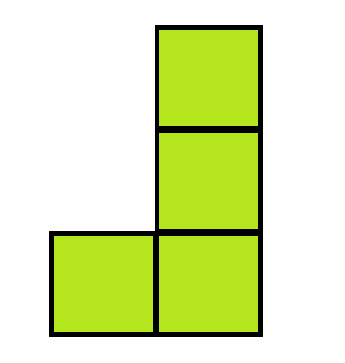
\includegraphics[width=2.05833in,height=2.16573in]{./imgSAEB_8_MAT/media/image57.png}
\end{figure}
\item 16x + 96
\item 4x^2 + 24x+ 144
\item 4x^2 + 48x+144
\item x^2 + 12x + 36

% SAEB: Identificar representações algébricas equivalentes.

% A: Incorreta, pois o aluno poderia, ao invés de realizar o cálculo da
% área, realizar o cálculo do perímetro.

% B: Incorreta, pois o aluno errou a multiplicação no termo ``x''.

% C: Correta, pois, considerando que cada lado dos quadrados tem (x+6), e
% que a área do quadrado é calculada pela fórmula l^2, temos que:

% (x+6) \cdot (x+6) =

% X^2 + 12x + 36

% Como temos 4 quadrados na figura:

% 4 \cdot (X^2 + 12x+ 36) =

% 4x^2 + 48x + 144.

% D: Incorreta, pois, caso o aluno considere calcular apenas 1 quadrado ao
% invés da figura toda, chegará a esse resultado erroneamente.

\num{7} Para representar a sua idade, Pedro utilizou a equação X^2 - 2 809 =
0. Sendo assim, qual é a idade real de Pedro? Resolver problemas que
possam ser representados por equações polinomiais de 2º grau.
\item 28 anos
\item 19 anos
\item 53 anos
\item 20 anos

% SAEB: Resolver uma equação polinomial de 2º grau.

% A: Incorreta, pois o aluno chegaria a essa conclusão ao considerar
% apenas uma parte da equação correspondente.

% B: Incorreta, pois o aluno chegaria a essa conclusão ao somar uma parte
% da equação correspondente, e não o resultado final.

% C: Correta, pois:

% Realizando as operações, obtemos:

% X^2 - 2 809 = 0

% X^2 = 2 809

% X= (\sqrt{2\ 809})

% X = 53

% D: Incorreta, pois o aluno chegaria a essa conclusão ao somar os
% elementos da equação correspondente, e não o resultado final.

\num{8} A China é um dos países mais populosos do mundo. Uma de suas regiões
tem uma população de 7.264 200. habitantes e ocupa uma área de 35.000
km^2. Qual é a densidade demográfica dessa região?
\item 207,5 Habitantes/km^2
\item 4,81 Habitantes/km^2
\item 2.075 Habitantes/km^2
\item 20 Habitantes/km^2

% SAEB: Calcular o resultado de adições, subtrações, multiplicações ou
% divisões envolvendo número reais.

% BNCC: EF08MA03 -- Resolver e elaborar problemas de contagem cuja
% resolução envolva a aplicação do princípio multiplicativo.

% A: Correta, pois, utilizando a razão da densidade demográfica -

% (densidade\ demografica = \frac{número\ de\ pessoas\ }{dimensão\ do\ espaço\ em\ km^2})
% -, temos que:

% (densidade\ demográfica = \frac{7\ 264\ 200}{35\ 000})

% (densidade\ demográfica = 207,5\ habitantes)/km^2

% B: Incorreta, pois o aluno, ao invés de realizar a divisão entre número
% de pessoas e dimensão do espaço em km^2, realizou a divisão da dimensão
% pelo número de pessoas.

% C: Incorreta, pois o aluno pode chegar a esse resultado cortando um
% ``zero'' a mais da expressão .

% D: Incorreta, pois o aluno pode chegar a esse resultado cortando um
% ``zero'' a menos da expressão.

\num{9} Um tijolo maciço comum possui aproximadamente 11 centímetros de
altura e 24 centímetros de comprimento. Para construir uma parede de sua
casa com o tamanho de 7 metros de largura e 4 de altura, Manoel comprou
1.500 tijolos. Essa quantidade foi suficiente?
\item Foi suficiente e sobrou 440 Tijolos
\item Foi suficiente e sobrou 1472 Tijolos
\item Não foi suficiente e Faltou 440 Tijolos
\item Manoel comprou tijolos necessários porem não houve sobra.

% SAEB: Construir/desenhar figuras geométricas planas ou espaciais que
% satisfaçam condições dadas.

% BNCC: EF08MA18 -- Reconhecer e construir figuras obtidas por composições
% de transformações geométricas (translação, reflexão e rotação), com o
% uso de instrumentos de desenho ou de softwares de geometria dinâmica.

% A: Correta, pois

% Calculando a parede da casa obtemos que a mesma possuirá 28m^2.

% Cada tijolo possui 0,11 \cdot 0,24 = 0,0264m^2 de área.

% Dividindo (28 \div 0,0264 = 1.060\; tijolos).

% Logo, 1500 - 1060 = 440 tijolos sobraram.

% B: Incorreta, pois o aluno chegaria a esse valor caso confundisse área
% com perímetro.

% C: Incorreta, pois o aluno, por meio de indução, pode ser levado a
% assinalá-la.

% D: Incorreta, pois o aluno pode assinalar a alternativa que pareça mais
% plausível para o enunciado.

\num{10} Na figura, AH é a altura e a bissetriz, relativa ao lado BC, do
triângulo ABC. Qual éa medida do ângulo x?

\begin{figure}[H]
\centering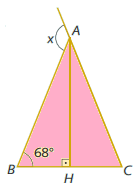
\includegraphics[width=1.45833in,height=2in]{./imgSAEB_8_MAT/media/image58.png}
\end{figure}
\item 136°
\item 22°
\item 44°
\item 68°

% SAEB: Resolver problemas que envolvam relações entre ângulos formados
% por retas paralelas cortadas por uma transversal, ângulos internos ou
% externos de polígonos ou cevianas (altura, bissetriz, mediana,
% mediatriz) de polígonos.

% A: Correta, pois, utilizando as informações da imagem, temos que

% 68 + 90 + ângulo BHA = 180

% 158 + ângulo BHA = 180

% Ângulo BHA = 22.

% Logo, como há uma bissetriz, temos que 22 + 22= 44°

% 180°- 44°= 136°.

% B: Incorreta, pois o aluno chegaria a essa conclusão calculando apenas o
% valor do ângulo BHA.

% C: Incorreta, pois o aluno chegaria a esse valor calculando apenas o
% valor da bissetriz do ângulo.

% D: Incorreta, pois o aluno chegaria a essa conclusão considerando o
% valor de outro ângulo diferente ao enunciado.

\num{11} Sabendo que a distância entre nossa cidade e outra localidade é de
1.235 km, e que pretendemos realizar uma viagem para esse destino em 30
dias, qual deslocamento diário mínimo devemos fazer?
\item 37 km por dia
\item 30 km por dia
\item 41 km por dia
\item 42 km por dia

% SAEB: Descrever ou esboçar deslocamento de pessoas e/ou de objetos em
% representações bidimensionais (mapas, croquis etc.), plantas de
% ambientes ou vistas, de acordo com condições dadas.

% A: pois, o aluno, ao invés de realizar uma divisão dos termos, pode
% realizar uma porcentagem, chegando a esse resultado erroneamente.

% B: Incorreta, pois o aluno pode chegar a essa conclusão confundindo o
% número de dias com a quantidade de kms a serem percorridos.

% C: Incorreta, pois o aluno chegaria a essa conclusão desconsiderando as
% casas decimais.

% D: Correta, pois

% 1.235km \div 30 dias = 41,16 km diários; logo, deveremos completar, no
% mínimo, 42 km por dia.

\num{12} Vicente Resolveu plantar girassóis em sua fazenda. Ao pesquisar os
últimos preços das sementes de girassóis, obteve os seguintes
resultados:

Janeiro: R\$\,12,25 kg Fevereiro: R\$\,13,40 kg Março: R\$\,12,95 kg Abril:
R\$\,11,25 kg Maio: R\$\,11,20kg Junho: R\$\,12,00 kg

Pode se dizer, então, que o preço médio das sementes de girassol nos
últimos 6 meses foi?
\item R\$\,12,17
\item R\$\,11,20
\item R\$\,13,40
\item R\$\,12,12

% SAEB: Calcular os valores de medidas de tendência central de uma
% pesquisa estatística (média aritmética simples, moda ou mediana).

% BNCC: EF08MA25 -- Obter os valores de medidas de tendência central de
% uma pesquisa estatística (média, moda e mediana) com a compreensão de
% seus significados e relacioná-los com a dispersão de dados, indicada
% pela amplitude.

% A: Correta, pois

% Somando os meses, obtemos: 73,05

% 73,05 \div 6 = 12,175.

% B: Incorreta, pois o aluno chegaria a esse resultado selecionando menor
% preço.

% C: Incorreta, pois o aluno chegaria a esse resultado selecionando o
% maior valor.

% D: Incorreta, pois o aluno chegaria a esse resultado calculando a
% mediana dos preços.

\num{13} Para concluir o projeto de sua pipa, qual é a quantidade em m^2 de
folha de seda que Mateus devera comprar?

\begin{figure}[H]
\centering
\includegraphics[width=1.45833in,height=1.63333in]{./imgSAEB_8_MAT/media/image59.png}
\end{figure}
\item 31,68 m^2
\item 15,84m^2
\item 11,6m^2
\item 1,63 m^2

% SAEB: Resolver problemas que envolvam medidas de grandezas (comprimento,
% massa, tempo, temperatura, capacidade ou volume) em que haja conversões
% entre unidades mais usuais.

% BNCC: EF08MA19 -- Resolver e elaborar problemas que envolvam medidas de
% área de figuras geométricas, utilizando expressões de cálculo de área
% (quadriláteros, triângulos e círculos), em situações como determinar
% medida de terrenos.

% A: Incorreta, pois o aluno chegará a esse valor caso considere
% multiplicar as duas diagonais em busca do valor da área.

% B: Correta, pois, utilizando a formula da área do losango, temos que:

% A=(\frac{\text{D\ .\ d}}{2})=

% A= (\frac{7,2\ .\ 4,4}{2})

% A= 15,84 m^2

% C: Incorreta, pois o aluno, ao invés de utilizar a fórmula do losango
% para definir a área, pode somar os valores.

% D: Incorreta, pois o aluno, ao invés de utilizar a fórmula do losango
% para definir a área, pode dividir os valores.

\num{14} Joana está tentando se cadastrar em um site de notícias. Ela deve
compor uma senha de acesso de 6 caracteres, dos quais os dois primeiros
devem ser vogais e os quatro últimos, algarismos de 0 a 9. Quantas
possibilidades de senha diferentes Joana pode criar? EF08MA22 -
\item 250.000 possibilidades
\item 25.000 possibilidades
\item 2.500 possibilidades
\item 250 possibilidades

% SAEB: Resolver problemas que envolvam a probabilidade de ocorrência de
% um resultado em eventos aleatórios equiprováveis independentes ou
% dependentes.

% A: Correta, pois, temos que o número de vogais do nosso alfabeto é 5,
% logo:

% 5 \cdot 5 \cdot 10 \cdot 10 \cdot 10 \cdot 10 = 250.000 possibilidades de senhas diferentes.

% B: Incorreta, pois, ao não considerar ``um elemento multiplicativo 10'',
% o aluno chegaria a essa conclusão erroneamente.

% C: Incorreta, pois, ao não considerar ``dois elementos multiplicativos
% 10'', o aluno chegaria a essa conclusão erroneamente.

% D: Incorreta, pois, ao não considerar ``três elementos multiplicativos
% 10'', o aluno chegaria a essa conclusão erroneamente.

\num{15} No plano cartesiano, considere o triângulo ABC com vértices A(2, 4),
B(5, 6) e C(7, 2). A figura obtida após aplicar uma transformação de
reflexão em relação ao eixo x nesse triângulo será:
\item Triângulo A'B'C' com vértices A'(-2, 4), B'(5, -6) e C'(7, -2).
\item Triângulo A'B'C' com vértices A'(-2, -4), B'(5, -6) e C'(7, -2).
\item Triângulo A'B'C' com vértices A'(-2, -4), B'(5, 6) e C'(7, 2).
\item Triângulo A'B'C' com vértices A'(2, -4), B'(-5, -6) e C'(-7, -2).

% SAEB: Identificar, no plano cartesiano, figuras obtidas por uma ou mais
% transformações geométricas (reflexão, translação, rotação).

% BNCC: EF08MA18 -- Reconhecer e construir figuras obtidas por composições
% de transformações geométricas (translação, reflexão e rotação), com o
% uso de instrumentos de desenho ou de softwares de geometria dinâmica.

% A: Incorreta, pois os valores dos vértices não condizem com o processo
% de reflexão.

% B: Correta, pois, ao realizar uma reflexão em relação ao eixo x, os
% pontos mantêm a mesma coordenada x, mas têm sua coordenada y negativa.
% No triângulo ABC original, o ponto A(2, 4) terá a mesma coordenada x,
% mas sua coordenada y será negativa, resultando em A'(-2, -4). Da mesma
% forma, os pontos B(5, 6) e C(7, 2) terão suas coordenadas y negativas
% após a reflexão, resultando em B'(5, -6) e C'(7, -2), respectivamente.

% C: Incorreta, pois os valores dos vértices não condizem com o processo
% de reflexão.

% D: Incorreta, pois os valores dos vértices não condizem com o processo
% de reflexão.

\num{16} Considere a tabela abaixo, que apresenta o número de livros vendidos
por três livrarias em um determinado mês:

%Paulo: criar uma tabela com as informações abaixo:

Livraria Número de Livros Vendidos Livraria A 120 Livraria B 80 Livraria
C 150

Com base nesses dados, assinale a alternativa correta:
\item A Livraria C vendeu mais livros do que a Livraria A e a Livraria B
juntas.
\item A Livraria A vendeu menos livros do que a Livraria B.
\item A Livraria C vendeu 70 livros a mais do que a Livraria A.
\item A Livraria B vendeu o dobro de livros em comparação com a Livraria C.

% SAEB: Resolver problemas que envolvam dados estatísticos apresentados em
% tabelas (simples ou de dupla entrada) ou gráficos (barras simples ou
% agrupadas, colunas simples ou agrupadas, pictóricos, de linhas, de
% setores ou em histograma).

% BNCC: EF08MA25 -- Obter os valores de medidas de tendência central de
% uma pesquisa estatística (média, moda e mediana) com a compreensão de
% seus significados e relacioná-los com a dispersão de dados, indicada
% pela amplitude.

% A: Incorreta, pois a Livraria C vendeu 150 livros, enquanto a Livraria A
% e a Livraria B juntas venderam 120 + 80 = 200 livros. Portanto, as
% livrarias A e B venderam mais livros do que a Livraria C.

% B: Incorreta, pois a Livraria A vendeu 120 livros, enquanto a Livraria B
% vendeu 80 livros. Portanto, a Livraria B vendeu menos livros do que a
% Livraria A.

% C: Incorreta, pois a diferença entre o número de livros vendidos pela
% Livraria C (150) e a Livraria A (120) é de 30 livros, e não 70 livros.

% D: Correta, pois a Livraria B vendeu 80 livros, enquanto a Livraria C
% vendeu 150 livros, e 150 é o dobro de 80.


\section*{Simulado 3}

\num{1} Em uma corrida, o primeiro lugar ganhou com diferença de 0,035 de
tempo para o segundo lugar. A diferença de tempo por extenso é:
\item~35 segundos
\item 35 milésimos de segundos
\item 35 centésimos de segundos~
\item 35 minutos

% SAEB: Escrever números racionais (representação fracionária ou decimal
% finita) em sua representação por algarismos ou em língua materna ou
% associar o registro numérico ao registro em língua materna.

% A: Incorreta, pois 35 segundos não é representado por números decimais.

% B: Correta, pois, quando há três casas decimais, temos milésimos de
% segundos.

% C: Incorreta, pois 35 centésimos de segundos apareceria com duas casas
% decimais após a vírgula.

% D: Incorreta, pois 3 minutos é uma quantidade representada por um número
% inteiro

\num{2} Marque a alternativa que classifica as seguintes variáveis,
respectivamente: Profissão, Batimentos cardíacos, Pressão, Altura.
\item Qualitativa, Quantitativa, Quantitativa, Quantitativa
\item Qualitativa, Qualitativa, Quantitativa, Quantitativa
\item Quantitativa, Qualitativa, Quantitativa, Quantitativa
\item Quantitativa, Quantitativa, Quantitativa, Quantitativa

% SAEB: Identificar os indivíduos (universo ou população-alvo da
% pesquisa), as variáveis e os tipos de variáveis (quantitativas ou
% categóricas) em um conjunto de dados.

% BNCC: EF08MA25 -- Obter os valores de medidas de tendência central de
% uma pesquisa estatística (média, moda e mediana) com a compreensão de
% seus significados e relacioná-los com a dispersão de dados, indicada
% pela amplitude.

% A: Correta, pois somente profissão não pode ser quantificada.

% B: Incorreta, pois batimentos cardíacos constituem uma variável
% quantitativa.

% C: Incorreta, pois profissão não é uma variável quantitativa e
% batimentos cardíacos não são qualitativos.

% D: Incorreta, pois profissão não é uma variável quantitativa.

\num{3} Em uma pesquisa qualitativa nominal, foram apresentados dados da cor
dos olhos da amostra escolhida. O gráfico era todo colorido dentro de um
círculo dividido em fatias. Qual tipo de gráfico é esse?

\begin{enumerate}
\def\labelenumi{\alph{enumi}.}
\item
  Histograma
\item
  Gráfico de barras
\item
  Gráfico de colunas
\item
  Gráfico de linhas~
\end{enumerate}

% SAEB: Representar ou associar os dados de uma pesquisa estatística ou de
% um levantamento em listas, tabelas (simples ou de dupla entrada) ou
% gráficos (barras simples ou agrupadas, colunas simples ou agrupadas,
% pictóricos, de linhas, de setores, ou em histograma).

% BNCC: EF08MA25 -- Obter os valores de medidas de tendência central de
% uma pesquisa estatística (média, moda e mediana) com a compreensão de
% seus significados e relacioná-los com a dispersão de dados, indicada
% pela amplitude.

% A: Incorreta, pois o histograma é feito por linhas e barras.

% B: Incorreta, pois o gráfico de barras é formado por barras retangulares
% e com base maior na horizontal.

% C: Correta, pois esse tipo de gráico apresenta setores de uma figura
% geométrica, geralmente, um círculo.

% D: Incorreta, pois o gráfico de linhas é representado por pontos unidos
% por linhas.

\num{4} Em um triângulo retângulo ABC, onde o ângulo B é reto, determine a
relação correta entre as medidas dos lados:
\item a^2 + b^2 = c^2 (Teorema de Pitágoras)
\item a + b = c (Propriedade da soma dos lados)
\item a = b (Lados congruentes em um triângulo retângulo)
\item a \textgreater{} b \textgreater{} c (Relação entre as medidas dos
lados)

% SAEB: Resolver problemas que envolvam relações métricas do triângulo
% retângulo, incluindo o teorema de Pitágoras.

% A: Correta, pois a^2 + b^2 = c^2 representa corretamente o Teorema de
% Pitágoras, que estabelece que, em um triângulo retângulo, o quadrado da
% hipotenusa (c) é igual à soma dos quadrados dos catetos (a e b).

% B: Incorreta, pois, na verdade, a soma dos quadrados dos catetos a e b é
% igual ao quadrado da hipotenusa c, como afirma o Teorema de Pitágoras.

% C: Incorreta, pois, em um triângulo retângulo, os lados a e b são os
% catetos, e eles podem ter medidas diferentes.

% D: Incorreta, pois não há uma relação específica entre as medidas dos
% lados a, b e c de um triângulo retângulo. As medidas podem variar
% dependendo do triângulo em questão.

\num{5} Julgue as afirmações e marque a resposta correta.

I - Todos os números inteiros são racionais.

II - Todo número decimal finito pode ser representado por fração.

III - O número 21 é primo.

IV - O número 2 é o único número que é par e primo.

\begin{enumerate}
\def\labelenumi{\alph{enumi})}
\item
  As questões II e IV são falsas.
\item
  I, II, e IV são verdadeiras.
\item
  Apenas IV é falsa.
\item
  São todas verdadeiras
\end{enumerate}

% SAEB: Converter uma representação de um número racional positivo para
% outra representação.

% A: Incorreta, pois todo número decimal finito pode ser representado por
% fração e o número 2 é o único par que é primo.

% B: Correta, pois essas são as afirmações certas.

% C: Incorreta, pois o número 2 é o único número par que é primo, então é
% uma verdade

% D: Incorreta, pois a afirmação III é falsa. O número 21 não é primo, ele
% possui 4 divisores: 1, 3,7 e 21.

\num{6} Ao analisar uma tabela de dupla entrada que apresenta a relação entre
o nível de escolaridade e a renda média mensal dos indivíduos, é
possível inferir a finalidade da pesquisa estatística realizada. Qual
das opções abaixo representa corretamente a finalidade dessa pesquisa?
\item Investigar a relação entre a idade e a renda dos indivíduos.
\item Comparar a escolaridade entre diferentes faixas etárias.
\item Identificar os fatores determinantes do nível de escolaridade.
\item Avaliar a influência da escolaridade na renda dos indivíduos.

% SAEB: Inferir a finalidade da realização de uma pesquisa estatística ou
% de um levantamento, dada uma tabela (simples ou de dupla entrada) ou
% gráfico, (barras simples ou agrupadas, colunas simples ou agrupadas,
% pictóricos, de linhas, de setores ou em histograma) com os dados dessa
% pesquisa.

% A: Incorreta, pois o gráfico não faz essa relação.

% B: Correta, pois o gráfica não apresenta faixas etárias.

% C: Incorreta, pois o gráfico não apresenta tais fatores.

% D: Correta, pois a tabela de dupla entrada apresenta a relação entre
% duas variáveis: o nível de escolaridade e a renda média mensal. A
% finalidade dessa pesquisa é analisar e inferir como o nível de
% escolaridade influencia a renda dos indivíduos. Ao cruzar os dados da
% tabela, é possível observar se há uma relação entre a escolaridade e a
% renda e, assim, avaliar a influência dessa variável na determinação da
% renda média mensal.

\num{7} Analise as afirmações e marque a correta.

I - A média é o valor que mais se repete.

II - Uma variável quantitativa pode ser expressa por números.

III - O primeiro passo para realizar uma pesquisa estatística é
delimitar o problema.
\item Apenas I está correta.
\item Todas estão erradas.
\item As afirmações II e III estão corretas.
\item As afirmações I e II estão corretas.

% SAEB: Interpretar o significado das medidas de tendência central (média,
% aritmética simples, moda e mediana) ou da amplitude.

% A: Incorreta, pois a I não está correta. mMédia, é a soma dos valores do
% conjunto de dados,dividido pela quantidade dos dados.

% B: Incorreta, pois somente a I está incorreta.

% C: Correta, pois a I é falsa. Moda é o valor que mais se repete.

% D: Incorreta, pois, a definição de moda está incorreta na I.

\num{8} Um prisma retangular possui 6 faces retangulares. Quantas arestas
esse prisma possui?
\item 8
\item 10
\item 12
\item 14

% SAEB: Relacionar o número de vértices, faces ou arestas de prismas ou
% pirâmides, em função do seu polígono da base.

% BNCC: EF08MA18 -- Reconhecer e construir figuras obtidas por composições
% de transformações geométricas (translação, reflexão e rotação), com o
% uso de instrumentos de desenho ou de softwares de geometria dinâmica.

% A: Incorreta, pois, se um prisma retangular tivesse 8 arestas, teria
% apenas duas arestas por face, o que não seria suficiente para formar as
% arestas laterais.

% B: Incorreta, pois, se um prisma retangular tivesse 10 arestas, teria
% três arestas por face, o que também não seria suficiente para formar as
% arestas laterais.

% C: Incorreta, pois, se um prisma retangular tivesse 12 arestas, teria
% quatro arestas por face, o que ainda não seria suficiente para formar as
% arestas laterais.

% D: Correta, pois um prisma retangular possui 12 arestas na base (4
% arestas do retângulo superior + 4 arestas do retângulo inferior + 4
% arestas verticais que conectam as bases). Além disso, existem duas
% arestas laterais que se estendem verticalmente e conectam os vértices
% das bases, totalizando 14 arestas.

\num{9} Qual das seguintes opções identifica corretamente a corda de uma
circunferência?
\item Um segmento de reta que liga dois pontos da circunferência.
\item Um segmento de reta que liga o centro da circunferência a um ponto
qualquer da circunferência.
\item Um arco da circunferência que possui a mesma medida que um ângulo
central.
\item Um segmento de reta que liga o centro da circunferência a um ponto
médio de um arco da circunferência.

% SAEB: Reconhecer circunferência/círculo como lugares geométricos, seus
% elementos (centro, raio, diâmetro, corda, arco, ângulo central, ângulo
% inscrito).

% BNCC: EF08MA18 -- Reconhecer e construir figuras obtidas por composições
% de transformações geométricas (translação, reflexão e rotação), com o
% uso de instrumentos de desenho ou de softwares de geometria dinâmica.

% A: Incorreta, pois uma corda não é apenas um segmento de reta que liga
% dois pontos da circunferência, já que não necessariamente passa pelo
% centro da circunferência.

% B: Incorreta, pois essa opção descreve o raio da circunferência, não a
% corda. O raio liga o centro da circunferência a um ponto específico na
% circunferência, enquanto a corda liga dois pontos quaisquer da
% circunferência.

% C: Incorreta, pois um arco da circunferência não pode ser considerado
% uma corda. A corda é um segmento de reta, enquanto o arco é uma parte da
% circunferência.

% D: Correta, pois a definição correta de uma corda é um segmento de reta
% que liga o centro da circunferência a um ponto médio de um arco da
% circunferência. Isso significa que a corda passa pelo centro da
% circunferência e divide o arco em duas partes iguais.

\num{10} Qual é o ponto médio do segmento de reta que tem as extremidades nos
pontos A(1, 2) e B(5, 6)?
\item (2, 4)
\item (3, 4)
\item (4, 5)
\item (5, 6)

% SAEB: Determinar o ponto médio de um segmento de reta ou a distância
% entre dois pontos quaisquer, dadas as coordenadas desses pontos no plano
% cartesiano.

% BNCC: EF08MA14 -- Demonstrar propriedades de quadriláteros por meio da
% identificação da congruência de triângulos.

% A: Incorreta, pois os valores obtidos após as operações não correspondem
% à alternativa.

% B: Correta, pois o ponto médio de um segmento de reta AB, cujas
% coordenadas dos pontos extremos são A(x1, y1) e B(x2, y2), é dado pelas
% coordenadas do ponto M(xm, ym), em que xm = (x1 + x2)/2 e ym = (y1 +
% y2)/2. Substituindo os valores dados na questão, temos: xm = (1 + 5)/2 =
% 3 e ym = (2 + 6)/2 = 4. Portanto, o ponto médio do segmento de reta AB é
% M(3, 4). As demais alternativas não correspondem às coordenadas do ponto
% médio.

% C: Incorreta, pois os valores obtidos após as operações não correspondem
% à alternativa.

% D: Incorreta, pois os valores obtidos após as operações não correspondem
% à alternativa.

\num{11} Qual das seguintes opções corretamente identifica as relações entre
as retas e segmentos de reta no plano cartesiano?
\item Duas retas são paralelas se possuem a mesma inclinação e intercepto y
diferente. Duas retas são perpendiculares se suas inclinações são
negativas inversas uma da outra.
\item Duas retas são concorrentes se possuem a mesma inclinação e
intercepto y diferente. Duas retas são paralelas se suas inclinações são
negativas inversas uma da outra.
\item Duas retas são perpendiculares se possuem inclinações iguais a zero e
interceptos y diferentes. Duas retas são paralelas se possuem
inclinações iguais e interceptos y diferentes.
\item Duas retas são paralelas se possuem inclinações iguais e interceptos
y diferentes. Duas retas são perpendiculares se suas inclinações são
negativas inversas uma da outra.

% SAEB: Identificar retas ou segmentos de retas concorrentes, paralelos ou
% perpendiculares.

% BNCC: EF08MA14 -- Demonstrar propriedades de quadriláteros por meio da
% identificação da congruência de triângulos.

% A: Incorreta, pois duas retas são paralelas se possuem a mesma
% inclinação e intercepto y iguais.

% B: Incorreta, pois duas retas são concorrentes se possuem inclinações
% diferentes, e duas retas são paralelas se possuem a mesma inclinação.

% C: Incorreta, pois duas retas podem ser paralelas sem ter inclinação
% igual a zero.

% D: Correta, duas retas são perpendiculares se a inclinação de uma é a
% negativa inversa da outra (isto é, seus coeficientes angulares
% multiplicados resultam em -1).

\num{12} Qual das alternativas abaixo representa a condição de existência de
um triângulo?
\item A soma dos ângulos internos é maior que 360 graus.
\item A medida de um dos ângulos internos é igual a 90 graus.
\item A medida do maior lado é igual a soma das medidas dos outros dois
lados.
\item A medida do menor lado é igual a metade da medida da hipotenusa.

% SAEB: Identificar propriedades e relações existentes entre os elementos
% de um triângulo (condição de existência, relações de ordem entre as
% medidas dos lados e as medidas dos ângulos internos, soma dos ângulos
% internos, determinação da medida de um ângulo interno ou externo).

% BNCC: EF08MA14 -- Demonstrar propriedades de quadriláteros por meio da
% identificação da congruência de triângulos.

% A: Incorreta, pois a soma dos ângulos internos de um triângulo é igual a
% 180 graus.

% B: Incorreta, pois, embora seja possível ter triângulos com um ângulo
% interno igual a 90 graus (triângulo retângulo), essa não é uma condição
% necessária para a existência de um triângulo.

% C: Correta, pois essa é uma regra aplicada aos triângulos.

% D: Incorreta, pois essa alternativa apresenta uma informação
% contraditória, pois a hipotenusa é o maior lado em um triângulo
% retângulo, portanto não pode ser menor que um dos outros lados. Além
% disso, não há relação definida entre a medida do menor lado e a da
% hipotenusa.

\num{13} Qual das alternativas abaixo classifica corretamente um triângulo em
relação aos seus lados?
\item Escaleno: possui todos os lados congruentes.
\item Isósceles: possui exatamente um par de lados congruentes.
\item Equilátero: possui exatamente dois lados congruentes.
\item Retângulo: não possui um ângulo interno reto.

% SAEB: Classificar triângulos ou quadriláteros em relação aos lados ou
% aos ângulos internos.

% BNCC: EF08MA14 -- Demonstrar propriedades de quadriláteros por meio da
% identificação da congruência de triângulos.

% A: Incorreta, pois um triângulo escaleno não possui lados congruentes.

% B: Correta, pois essa é a definição de um triângulo isósceles.

% C: Incorreta, pois um triângulo equilátero possui todos os lados
% congruentes.

% D: Incorreta, pois triângulo retângulo possui um ângulo interno reto.

\num{14} Em um triângulo, se um ângulo mede 90 graus, quanto mede a soma dos
outros dois ângulos?
\item 60 graus
\item 90 graus
\item 100 graus
\item 180 graus

% SAEB: Identificar relações entre ângulos formados por retas paralelas
% cortadas por uma transversal.

% BNCC: EF08MA14 -- Demonstrar propriedades de quadriláteros por meio da
% identificação da congruência de triângulos.

% A: Incorreta, pois o aluno errou na soma dos ângulos.

% B: Incorreta, pois o aluno não soube aplicar a soma dos ângulos
% internos.

% C: Incorreta, pois o aluno não somou 80º para encontrar o resultado
% correto.

% D: Correta, pois a soma dos ângulos internos de um triângulo é sempre
% igual a 180 graus. Se um dos ângulos mede 90 graus, a soma dos outros
% dois ângulos deve ser igual a 180 - 90 = 90 graus.

\num{15} Um terreno tem formato retangular e sua largura mede 20m. Um outro
terreno, que é uma ampliação do primeiro, tem formato retangular também
e sua largura mede 30m. Se o comprimento do primeiro terreno é de 40m,
qual é o comprimento do segundo terreno?
\item 60 m
\item 80 m
\item 120 m
\item 150 m

% SAEB: Resolver problemas que envolvam polígonos semelhantes.

% BNCC: EF08MA14 -- Demonstrar propriedades de quadriláteros por meio da
% identificação da congruência de triângulos.

% A: Incorreta, pois essa é a metade do comprimento do primeiro terreno, o
% que não condiz com a proporção estabelecida entre os terrenos.

% B: Incorreta, pois essa é uma opção que poderia ser confundida com a
% resposta correta, já que é um múltiplo do comprimento do primeiro
% terreno. No entanto, não corresponde à proporção estabelecida entre os
% terrenos.

% C: correta, pois sabemos que os terrenos são semelhantes, logo, os lados
% correspondentes são proporcionais. Como a largura do segundo terreno é
% 1,5 vezes maior do que a largura do primeiro (30 m/20 m), podemos
% afirmar que o comprimento do segundo terreno é 1,5 vezes maior do que o
% comprimento do primeiro terreno.

% D: Incorreta, pois essa é uma opção que poderia ser confundida com a
% resposta correta, já que é um múltiplo da largura do segundo terreno. No
% entanto, não corresponde à proporção estabelecida entre os terrenos.

\num{16} Um objeto é lançado verticalmente para cima a partir do solo, com
uma velocidade inicial de 30 metros por segundo. O objeto é afetado pela
força da gravidade, que causa uma aceleração constante de -9,8 metros
por segundo ao quadrado. Qual das seguintes equações polinomiais de 2º
grau modela corretamente a altura h (em metros) do objeto em relação ao
tempo t (em segundos)?
\item h(t) = -9,8t^2 + 30t
\item h(t) = -9,8t^2 - 30t
\item h(t) = 9,8t^2 - 30t
\item h(t) = 9,8t^2 + 30t

% SAEB: Inferir uma equação polinomial de 2º grau que modela um problema.

% BNCC: EF08MA09 -- Resolver e elaborar, com e sem uso de tecnologias,
% problemas que possam ser representados por equações polinomiais de 2º
% grau do tipo ax^2 = b.

% A: Correta, pois a combinação dos termos -9,8t^2 e 30t representa
% corretamente a queda da altura do objeto devido à gravidade e o aumento
% inicial da altura com a velocidade inicial de lançamento.

% B: Incorreta, pois o sinal negativo em ambos os termos não representa
% corretamente o comportamento do objeto em relação à altura.

% C: Incorreta, pois o sinal positivo em ambos os termos não representa
% corretamente o comportamento do objeto em relação à altura.

% D: Incorreta, pois o sinal positivo em ambos os termos não representa
% corretamente o comportamento do objeto em relação à altura.


\section*{Simulado 4}

\num{1} Uma cerca retangular tem 10 metros de comprimento e 6 metros de
largura. Qual é o perímetro da cerca?
\item 16 m
\item 22 m
\item 32 m
\item 60 m

% SAEB: Resolver problemas que envolvam perímetro de figuras planas.

% A: Incorreta, pois, ao aplicar a fórmula do perímetro, chegamos a um
% resultado diferente.

% B: Incorreta, pois, ao aplicar a fórmula do perímetro, chegamos a um
% resultado diferente.

% C: Correta, pois, no caso da cerca retangular descrita na questão, temos
% que ``a'' = 10 metros e ``b'' = 6 metros. Então, podemos calcular o
% perímetro da seguinte maneira:

% P = 2a + 2b P = 2(10) + 2(6) P = 20 + 12 P = 32

% D: Incorreta, pois, ao aplicar a fórmula do perímetro, chegamos a um
% resultado diferente.

\num{2} Quais são os passos para a realização de uma pesquisa estatística?
\item Definição do problema, seleção da amostra, coleta de dados, análise
dos dados, conclusões e recomendações.
\item Seleção da amostra, definição do problema, coleta de dados, análise
dos dados, conclusões e recomendações.
\item Coleta de dados, definição do problema, análise dos dados, seleção da
amostra, conclusões e recomendações.
\item Análise dos dados, coleta de dados, definição do problema, seleção da
amostra, conclusões e recomendações.

% SAEB: Explicar/descrever os passos para a realização de uma pesquisa
% estatística ou de um levantamento.

% BNCC: EF08MA25 -- Obter os valores de medidas de tendência central de
% uma pesquisa estatística (média, moda e mediana) com a compreensão de
% seus significados e relacioná-los com a dispersão de dados, indicada
% pela amplitude.

% A: Correta, pois essa é a ordem correta de uma pesquisa estatística.

% B: Incorreta, pois o primeiro passo está na posição 2.

% C: Incorreta, pois o primeiro passo está na posição 2.

% D: Incorreta, pois o primeiro passo está na posição 3.

\num{3} As notas de Geografia de 20 alunos foram colocadas na tabela abaixo:

%Paulo: Criar uma tabela com as informações a seguir:

\begin{longtable}[]{@{}llllllllll@{}}
\toprule
7,0 & 5,0 & 9,0 & 5,0 & 8,0 & 5,0 & 8,0 & 9,0 & 10,0 &
8,0\tabularnewline
\midrule
\endhead
6,0 & 6,0 & 7,0 & 7,0 & 7,0 & 5,0 & 5,0 & 5,0 & 6,0 & 6,0\tabularnewline
\bottomrule
\end{longtable}

Quantos alunos obtiveram nota maior ou igual a 7,0?
\item 8
\item 10
\item 9
\item 11

% SAEB: Argumentar ou analisar argumentações/conclusões com base nos dados
% apresentados em tabelas (simples ou de dupla entrada) ou gráficos
% (barras simples ou agrupadas, colunas simples ou agrupadas, pictóricos,
% de linhas, de setores ou em histograma).

% BNCC: EF08MA25 -- Obter os valores de medidas de tendência central de
% uma pesquisa estatística (média, moda e mediana) com a compreensão de
% seus significados e relacioná-los com a dispersão de dados, indicada
% pela amplitude.

% A: Incorreta, pois, ao visualizar 2 valores a menos do que realmente
% está na tabela, o aluno chegará a essa conclusão erroneamente.

% B: Correta, pois entre as notas fornecidas, temos 10 notas maiores ou
% iguais a 7,0.

% C: Incorreta, pois, ao visualizar 1 valor a menos do que realmente está
% na tabela, o aluno chegará a essa conclusão erroneamente.

% D: Incorreta, pois, ao visualizar 1 valor a mais do que realmente está
% na tabela, o aluno chegará a essa conclusão erroneamente.

\num{4} Deseja-se pregar uma fita decorativa ao redor da tampa de um pote
redondo. Se o diâmetro da tampa mede 12 cm, qual é o comprimento mínimo
que a fita deve ter para dar a volta completa nela?

Considere π = 3
\item 72 cm
\item 108 cm
\item 35 cm
\item 11 cm

% SAEB: Resolver problemas que envolvam relações entre os elementos de uma
% circunferência/círculo (raio, diâmetro, corda, arco, ângulo central,
% ângulo inscrito).

% BNCC: EF08MA18 -- Reconhecer e construir figuras obtidas por composições
% de transformações geométricas (translação, reflexão e rotação), com o
% uso de instrumentos de desenho ou de softwares de geometria dinâmica.

% A: Incorreta, pois o aluno pode esquecer que o valor do raio é a metade
% do diâmetro, chegando nesse valor.

% B: Incorreta, pois ao confundir a fórmula do perímetro da circunferência
% com a fórmula da área da circunferência chegará a esse valor.

% C: Incorreta, pois, ao realizar uma soma ao invés de uma multiplicação
% na fórmula, obterá esse valor.

% D: Correta, pois ao considerar pi = 3, temos que 2.3.6 = 36 cm

\num{5} Qual das seguintes afirmações é verdadeira sobre polígonos
semelhantes?
\item Dois polígonos são semelhantes se têm o mesmo número de lados.
\item Dois polígonos são semelhantes se têm ângulos correspondentes
congruentes e lados correspondentes proporcionais.
\item Dois polígonos são semelhantes se têm a mesma medida de área.
\item Dois polígonos são semelhantes se têm os mesmos comprimentos de lado.

% SAEB: Reconhecer polígonos semelhantes ou as relações existentes entre
% ângulos e lados correspondentes nesses tipos de polígonos.

% BNCC: EF08MA18 -- Reconhecer e construir figuras obtidas por composições
% de transformações geométricas (translação, reflexão e rotação), com o
% uso de instrumentos de desenho ou de softwares de geometria dinâmica.

% A: Incorreta, pois o número de lados não é suficiente para determinar se
% dois polígonos são semelhantes.

% B: Correta, pois dois polígonos são semelhantes se, ao sobrepor um sobre
% o outro, as medidas de seus lados correspondentes são multiplicadas por
% uma mesma constante de proporcionalidade.

% C: Incorreta, pois mesmo que dois polígonos tenham áreas iguais, eles
% não necessariamente são semelhantes.

% D: Incorreta, pois dois polígonos podem ter os mesmos comprimentos de
% lado, mas não serem semelhantes.

\num{6} Considere um polígono com 7 lados. É correto afirmar que:
\item É um polígono regular.
\item É um polígono não regular.
\item É um polígono regular ou não regular, dependendo da medida dos seus
lados.
\item É um polígono regular ou não regular, dependendo da medida de seus
ângulos internos

% SAEB: Classificar polígonos em regulares e não regulares.

% BNCC: EF08MA18 -- Reconhecer e construir figuras obtidas por composições
% de transformações geométricas (translação, reflexão e rotação), com o
% uso de instrumentos de desenho ou de softwares de geometria dinâmica.

% A: é Incorreta, pois o polígono não possui lados e ângulos congruentes.

% B: Correta, pois essa é uma das características do polígono.

% C: é Incorreta, pois a medida dos lados não influencia na classificação
% do polígono como regular ou não regular.

% D: é Incorreta, pois mesmo que os ângulos internos do polígono sejam
% congruentes, ainda assim é impossível que seus lados sejam congruentes.

\num{7} Qual das alternativas abaixo associa corretamente uma equação
polinomial de 1º grau com duas variáveis a uma reta no plano cartesiano?
\item y = 2x - 3 corresponde a uma reta com inclinação 2 e intercepto no
eixo y de -3.
\item y = -3x + 2 corresponde a uma reta com inclinação -3 e intercepto no
eixo x de 2.
\item y = 4x + 1 corresponde a uma reta com inclinação 1/4 e intercepto no
eixo y de 1.
\item y = -x - 5 corresponde a uma reta com inclinação -1 e intercepto no
eixo y de -5.

% SAEB: Associar uma equação polinomial de 1º grau com duas variáveis a
% uma reta no plano cartesiano.

% BNCC: EF08MA07 -- Associar uma equação linear de 1º grau com duas
% incógnitas a uma reta no plano cartesiano.

% A: Correta, pois uma equação polinomial de 1º grau com duas variáveis,
% na forma y = ax + b, representa uma reta no plano cartesiano. O
% coeficiente a é a inclinação da reta e o coeficiente b é o intercepto no
% eixo y. Assim, podemos associar a equação y = 2x - 3 com a reta que
% passa pelo ponto (0, -3) e tem inclinação 2. A inclinação positiva
% indica que a reta sobe da esquerda para a direita no plano cartesiano. O
% intercepto no eixo y indica que a reta cruza o eixo y no ponto (0, -3

% B: Incorreta, pois alternativa apresenta uma equação com inclinação
% negativa.

% C: Incorreta, pois a alternativa apresenta uma equação com inclinação
% diferente de 1.

% D: Incorreta, pois a alternativa apresenta uma equação com inclinação
% diferente de 1.

\num{8} Para cobrir 840 m^2 de um telhado, 14 operários, que apresentam a
mesma produtividade, gastam 7 horas. Para cobrir outros 3.360 m^2 do
telhado, foram contratados outros 14 operários, que também possuem a
mesma produtividade individual dos operários anteriores. A previsão de
tempo que esses 12 operários gastariam para realizar esse trabalho É de
\item 3 horas e 30 minutos.
\item 7 horas.
\item 14 horas.
\item 18 horas e 10 minutos.

% SAEB: Inferir uma equação, inequação polinomial de 1º grau ou um sistema
% de equações de 1º grau com duas incógnitas que modela um problema.

% BNCC: EF08MA07 -- Associar uma equação linear de 1º grau com duas
% incógnitas a uma reta no plano cartesiano.

% Alternativa A: Incorreta, pois ,ao realizar incorretamente a montagem da
% regra de 3, o aluno chegará a esse valor incorreto.

% Alternativa B: Incorreta, pois, ao realizar incorretamente a
% multiplicação do resultado final por 2, o aluno chegará a esse resultado
% equivocadamente.

% Alternativa C: Correta, pois, ao realizarmos a regra de três
% (\frac{14}{7} \cdot \frac{28}{x}), levando em conta os outros 3.360 m^2,
% chegamos a 14 horas.

% Alternativa D: Incorreta, pois, ao realizar incorretamente a montagem da
% regra de 3, o aluno chegará a esse valor incorreto.

\num{9} Em uma padaria, há uma torta que pode ser dividida em 8 pedaços
iguais. João comeu 3 desses pedaços, e Maria comeu 2/4 da torta. Quem
comeu mais torta?
\item João
\item Maria
\item João e Maria comeram a mesma quantidade de torta
\item Não é possível determinar a resposta, pois as frações são diferentes.

% SAEB: Representar frações menores ou maiores que a unidade por meio de
% representações pictóricas ou associar frações a representações
% pictóricas.

% BNCC: EF08MA05 -- Reconhecer e utilizar procedimentos para a obtenção de
% uma fração geratriz para uma dízima periódica.

% A: Incorreta, pois o aluno provavelmente efetuou a operação de maneira
% incorreta.

% B: Correta, pois
% (\frac{2}{4} = \frac{(2 \cdot 2)} {(4 \cdot 2)} = \frac{4}{8} > \frac{3}{8})
% logo, Maria comeu mais torta.

% C: Incorreta, pois a operação demonstra que Maria e João comeram porções
% diferentes.

% D: Incorreta, pois o aluno deve saber comparar frações diferentes.

\num{10} Dois corredores saem da linha de partida ao mesmo tempo. Sabendo que
um deles percorre toda a pista em 15 minutos e o outro, em 25 minutos,
dentro de quanto tempo eles se encontram novamente na linha de partida?
\item 5 minutos b) 40 minutos. c) 1 hora e 5 minutos d) 1 hora e 15 minutos

% SAEB: Resolver problemas que envolvam as ideias de múltiplo, divisor,
% máximo divisor comum ou mínimo múltiplo comum.

% BNCC: EF08MA02 -- Resolver e elaborar problemas usando a relação entre
% potenciação e radiciação, para representar uma raiz como potência de
% expoente fracionário.

% A: Incorreta, pois considerou que o tempo de encontro seria pelo M.D.C
% ao invés do M.M.C. .

% B: Incorreta, pois apenas foi feita a soma do tempo de cada corredor.

% C: Incorreta, pois foi associado um número errado de minutos.

% D: Correta, pois devemos usar a ideia de mínimo múltiplo comum. Assim,
% calculando o M.M.C dos tempos, temos:

\num{11} As notas de Geografia de 20 alunos foram colocadas na tabela abaixo:

%Paulo: Criar uma tabela com as informações a seguir:

\begin{longtable}[]{@{}llllllllll@{}}
\toprule
7,0 & 5,0 & 9,0 & 5,0 & 8,0 & 5,0 & 8,0 & 9,0 & 10,0 &
8,0\tabularnewline
\midrule
\endhead
6,0 & 6,0 & 7,0 & 7,0 & 7,0 & 5,0 & 5,0 & 5,0 & 6,0 & 6,0\tabularnewline
\bottomrule
\end{longtable}

Quantos alunos obtiveram nota maior ou igual a 7,0?
\item 8
\item 10
\item 9
\item 11

% SAEB: Argumentar ou analisar argumentações/conclusões com base nos dados
% apresentados em tabelas (simples ou de dupla entrada) ou gráficos
% (barras simples ou agrupadas, colunas simples ou agrupadas, pictóricos,
% de linhas, de setores ou em histograma).

% BNCC: EF08MA25 -- Obter os valores de medidas de tendência central de
% uma pesquisa estatística (média, moda e mediana) com a compreensão de
% seus significados e relacioná-los com a dispersão de dados, indicada
% pela amplitude.

% A: Incorreta, pois, ao visualizar 2 valores a menos do que realmente
% está na tabela, o aluno chegará a essa conclusão erroneamente.

% B: Correta, pois entre as notas fornecidas, temos 10 notas maiores ou
% iguais a 7,0.

% C: Incorreta, pois, ao visualizar 1 valor a menos do que realmente está
% na tabela, o aluno chegará a essa conclusão erroneamente.

% D: Incorreta, pois, ao visualizar 1 valor a mais do que realmente está
% na tabela, o aluno chegará a essa conclusão erroneamente.

\num{12} Calcule o valor da expressão: 3^2 + raiz quadrada de 16.
\item 13
\item 11
\item 7
\item 10

% SAEB: Calcular o resultado de potenciação ou radiciação envolvendo
% números reais.

% BNCC: EF08MA02 -- Resolver e elaborar problemas usando a relação entre
% potenciação e radiciação, para representar uma raiz como potência de
% expoente fracionário.

% Alternativa A: Incorreta, pois a resolução da expressão não corresponde
% a esse resultado.

% Alternativa B: Incorreta, pois a resolução da expressão não corresponde
% a esse resultado.

% Alternativa C: Incorreta, pois a resolução da expressão não corresponde
% a esse resultado.

% Alternativa D: correta pois 3^2 significa 3 elevado ao quadrado, ou seja,
% 3 \cdot 3 = 9. (\sqrt 16) é 4. Assim, a expressão pode ser reescrita como
% 9 + 4 = 13.

\num{13} O maior cometa já descoberto é o Holmes, que possui 2.251 km de
diâmetro. Quantas classes possui o número que representa o diâmetro do
cometa?
\item 3
\item 2
\item 2.251
\item 4

% SAEB: Compor ou decompor números racionais positivos (representação
% decimal finita) na forma aditiva, ou em suas ordens, ou em adições e
% multiplicações.

% A: Incorreta, pois, caso o aluno resolva transformar km em m, esse seria
% o valor, mas não é isso que o enunciado pede.

% B: Correta, pois O número 2.251 possui 2 classes e 4 ordens.

% C: Incorreta, pois o aluno pode considerar que o numeral signifique o
% valor da classe, o que está incorreto.

% D: Incorreta, pois o aluno pode confundir classes com ordens.

\num{14} Qual a forma correta de escrever o número 49 em numeração romana?
\item XLVIX
\item LIXV
\item XLIX
\item XLIVIX

% SAEB: Comparar ou ordenar números reais, com ou sem suporte da reta
% numérica, ou aproximar número reais para múltiplos de potência de 10
% mais próxima.

% A: Incorreta, pois o aluno pode chegar a essa conclusão esquecendo que
% que no sistema romano são apenas em casos específicos de impossibilidade
% de colocar mais de 3 símbolos iguais para representar o mesmo número
% para inserir um número antes de outro representando uma subtração
% momentânea.

% B: Incorreta, pois o aluno pode chegar a essa conclusão esquecendo que
% que no sistema romano são apenas em casos específicos de impossibilidade
% de colocar mais de 3 símbolos iguais para representar o mesmo número
% para inserir um número antes de outro representando uma subtração
% momentânea.

% C: Correta, pois

% 40 = XL

% 9 = IX

% XLIX = 40 + 9 = 49

% D: Incorreta, pois o aluno pode chegar a essa conclusão esquecendo que
% que no sistema romano são apenas em casos específicos de impossibilidade
% de colocar mais de 3 símbolos iguais para representar o mesmo número
% para inserir um número antes de outro representando uma subtração
% momentânea.

\num{15} Amanda abastece seu veículo a cada 5 dias, Carlos a cada 2 dias.
Paulo vai abastecer seu veículo sempre aos sábados e em nenhum outro
dia. Se no dia 28 de outubro os três abasteceram seus veículos, daqui a
quantos dias eles abastecerão, novamente, no mesmo dia?
\item 31 dias
\item 25 dias
\item 70 dias
\item esse evento nunca mais acontecerá.

% SAEB: Identificar um número natural como primo, composto,
% ``múltiplo/fator de'' ou ``divisor de'' ou identificar a decomposição de
% um número natural em fatores primos ou relacionar as propriedades
% aritméticas (primo, composto, ``múltiplo/fator de'' ou ``divisor de'')
% de um número natural à sua decomposição em fatores primos.

% A: Incorreta, pois, por questão de semelhança, o aluno pode considerar
% que as 3 pessoas citadas no enunciado abastecerão sempre no mesmo dia 28
% de todo mês.

% B: Incorreta, pois o aluno pode realizar uma soma dos dias ao invés de
% realizar o m.m.c.

% C: Correta, pois

% MMC(5;7,2) = 70

% D: Incorreta, pois o aluno pode confundir m.m.c. por m.d.c.